\documentclass[a0paper, portrait]{baposter}

\usepackage{setspace}
\usepackage{multicol}
\usepackage[overlay]{textpos}
\setlength{\TPHorizModule}{10mm}
\setlength{\TPVertModule}{\TPHorizModule}

\usepackage[T1]{fontenc}
\usepackage[utf8]{inputenc}
\usepackage{lmodern}
\usepackage{bold-extra}
\usepackage{multicol}
\usepackage[numbers]{natbib}
\usepackage[strings]{underscore}

\usepackage{enumitem}
\setlist{nolistsep}

\RequirePackage{xspace}
\RequirePackage{relsize} % for \smaller
\RequirePackage{amsmath}
\RequirePackage{amssymb}
\RequirePackage{qrcode}

\RequirePackage{tikz}
\usetikzlibrary{arrows}
\usetikzlibrary{calc}
\usetikzlibrary{chains}
\usetikzlibrary{fadings}
\usetikzlibrary{fit}
\usetikzlibrary{positioning}
\usetikzlibrary{shapes}
\usetikzlibrary{backgrounds}
\usetikzlibrary{shapes.callouts}
\usetikzlibrary{arrows}
\usetikzlibrary{arrows.meta}
\pgfdeclarelayer{foreground}
\pgfsetlayers{background,main,foreground}


\definecolor{ftsrg@White}{RGB}{255,255,255}
\definecolor{ftsrg@Black}{RGB}{0,0,0}
\definecolor{ftsrg@Gray}{RGB}{167,168,167}
\definecolor{ftsrg@DarkGray}{RGB}{47,45,46}
\definecolor{ftsrg@AccentBlue}{RGB}{20,70,160}
\definecolor{ftsrg@AccentRed}{RGB}{150,0,24}
\definecolor{ftsrg@AccentPurple}{RGB}{82,43,71}
\definecolor{ftsrg@AccentOrange}{RGB}{251,139,36}
\definecolor{ftsrg@AccentLightBlue}{RGB}{68,114,196}
\definecolor{ftsrg@AccentGreen}{RGB}{112,173,71}

% These are for beamer-compatibility (best-effort)
\usepackage{tcolorbox}
\tcbuselibrary{skins,breakable}

\newenvironment{block}[1]{%
\tcolorbox[%
boxsep=1pt,left=0pt,right=0pt,top=3pt,bottom=3pt,%
colbacktitle=ftsrg@AccentBlue,
boxrule=0pt,
bottomtitle=1pt,toptitle=1pt,
frame hidden,
enhanced jigsaw,
noparskip,breakable,%
colback=ftsrg@DarkGray!10,%
title=#1]}%
{\endtcolorbox}

\newenvironment{columns}[1][]
        {\setkeys{columns@col}{#1}
         \noindent\begin{minipage}{\textwidth}}
        {\end{minipage}\vspace{.5cm}}

\newenvironment{column}[1]
        {\begin{minipage}[t]{#1}}
        {\end{minipage}}

\usepackage{listings}
\usepackage{caption}
\usepackage{subcaption}
\usepackage{algorithm}
\usepackage{algpseudocode}
\usepackage{amsthm}
\usepackage{amsfonts}
\usepackage{graphicx}

\usepackage{amsmath}
\usepackage{orcidlink}
\usepackage{tikz}
\usetikzlibrary{arrows,shapes,decorations,patterns,calc}
\usepackage{booktabs}


\usepackage{array}
\usepackage{collect}

\newcommand{\po}{\emph{po}}
\newcommand{\ppo}{{\color{gray}\emph{ppo}}}
\newcommand{\rf}{{\color{red}\emph{rf}}}
\newcommand{\fr}{{\color{cyan}\emph{fr}}}
\newcommand{\co}{{\color{orange}\emph{co}}}
\newcommand{\hb}{{\bfseries\emph{hb}}}


\newcounter{litmus}[section]

\newcommand{\litmusautorefname}{Program}

\newenvironment{litmus}[4]
{%
  \def\closing{#4}%
  \renewcommand\thelitmus{#2}%
  \refstepcounter{litmus}%
  \label{litmus:#2}%
  \begin{equation*}%
  \begin{gathered}%
  #3\\%
  \ifcase#1%
    \PackageError{litmus}{Invalid parameter value for array}{%
      The parameter value must be between 1 and 3.%
    }%
  % case 1
  \or
    \PackageError{litmus}{Invalid parameter value for array}{%
      The parameter value must be between 1 and 3.%
    }%
  % case 2
  \or
    \begin{array}{
      >{\displaystyle}l   % right aligned
      @{\hspace{1em}}     % spacing
      |                   % vertical rule
      @{\hspace{1em}}     % spacing
      >{\displaystyle}l   % left aligned
    }%
  % case 3
  \or
    \begin{array}{
      >{\displaystyle}r   % right aligned
      @{\hspace{1em}}     % spacing
      |                   % vertical rule
      @{\hspace{1em}}     % spacing
      >{\displaystyle}l   % left aligned
      @{\hspace{1em}}     % spacing
      |                   % vertical rule
      @{\hspace{1em}}     % spacing
      >{\displaystyle}l   % left aligned
    }%
  % case 4
  \or
    \begin{array}{
      >{\displaystyle}r   % right aligned
      @{\hspace{1em}}     % spacing
      |                   % vertical rule
      @{\hspace{1em}}     % spacing
      >{\displaystyle}l   % left aligned
      @{\hspace{1em}}     % spacing
      |                   % vertical rule
      @{\hspace{1em}}     % spacing
      >{\displaystyle}l   % left aligned
      @{\hspace{1em}}     % spacing
      |                   % vertical rule
      @{\hspace{1em}}     % spacing
      >{\displaystyle}l   % left aligned
    }%
  % default case
  \else
    \PackageError{litmus}{Invalid parameter value for array}{%
      The parameter value must be between 1 and 3.%
    }%
  \fi%
}{%
  \end{array}%
  \\\closing{}\end{gathered}%
  \end{equation*}%
}
 
\newcommand{\x}{\mathbf{x}}
\newcommand{\y}{\mathbf{y}}
\newcommand{\z}{\mathbf{y}}
\newcommand{\w}{\mathbf{y}}

\definecolor{po_color}{HTML}{000000}
\definecolor{ppo_color}{HTML}{2b83ba}
\definecolor{rf_color}{HTML}{d7191c}
\definecolor{fr_color}{HTML}{fdae61}
\definecolor{co_color}{HTML}{fdae61}
\definecolor{ext_color}{HTML}{000000}

\newcounter{threadnum}
\newcounter{threaddepth}
\newcounter{legendcnt}
\definecollection{initialwrites}
\definecollection{edges}
\definecollection{legend}


\newenvironment{execgraph}[1][0.75]
{%
\setcounter{threadnum}{0}
\setcounter{legendcnt}{0} \begin{collect}{legend}{}{} \end{collect}
\begin{tikzpicture}[scale=#1, x=1.5cm, y=1.25cm, every node/.style={transform shape}]
\tikzset{vertex/.style = {shape=ellipse,minimum size=1.5em,color=black}}
\tikzset{po_edge/.style = {->,> = latex',color=po_color}}
\tikzset{co_edge/.style = {->,> = latex',color=co_color}}
\tikzset{ppo_edge/.style = {->,> = latex',color=ppo_color}}
\tikzset{rf_edge/.style = {->,> = latex',color=rf_color}}
\tikzset{fr_edge/.style = {->,> = latex',color=fr_color}}
\tikzset{ext_edge/.style = {-,> = latex',color=ext_color}}
\tikzset{
    cross/.style={
      decoration={
        markings,
        mark=at position 0.5 with {
          \draw[-,solid] (-2pt,-2pt) -- (2pt,2pt);
          \draw[-,solid] (-2pt,2pt) -- (2pt,-2pt);
        }
      },
      postaction={decorate}
    }
  }
}%
{
\node[vertex] (init) at  (${\thethreadnum-1}*(0.5,0)$){\includecollection{initialwrites}};
\node[minimum height=0, minimum width=0, inner sep=0] (legend) at  (${\thethreadnum-1}*(0.5,0)$){%
\begin{tikzpicture}[scale=1, x=1cm, y=1cm, every node/.style={transform shape}]
      \node[] at (0,-1.5) {};
      \includecollection{legend}
    \end{tikzpicture}};
\includecollection{edges}
\end{tikzpicture}
}

\newenvironment{thread}
{%
\setcounter{threaddepth}{0}
}%
{\stepcounter{threadnum}}


\newcommand{\IW}[2]{\begin{collect}{initialwrites}{}{}$#1 := #2$\end{collect}}

\newcommand{\W}[3]{\stepcounter{threaddepth}\node[vertex] (#1) at  (\thethreadnum,-\thethreaddepth) {$#2 := #3$};}
\newcommand{\R}[3]{\stepcounter{threaddepth}\node[vertex] (#1) at  (\thethreadnum,-\thethreaddepth) {$#3 := #2$};}

\newcommand{\edge}[4]{\begin{collect}{edges}{}{}\draw[#1_edge] (#2) edge #4 (#3);\end{collect}}
\newcommand{\edgeL}[5]{\begin{collect}{edges}{}{}\draw[#1_edge] (#2) edge [bend left=#5] #4 (#3);\end{collect}}
\newcommand{\edgeR}[5]{\begin{collect}{edges}{}{}\draw[#1_edge] (#2) edge [bend right=#5] #4 (#3);\end{collect}}

\newcommand{\legend}[1]{\begin{collect}{legend}{}{}\node[] (\thelegendcnt) at (\thelegendcnt,0) {};\draw[#1_edge] (\thelegendcnt) edge node[above=0.25cm] {\emph{#1}} ($\thelegendcnt*(1,0) + (0.75,0)$);\stepcounter{legendcnt}\end{collect}} % remove this if not weak memory-related

% we define our own URL-format, because
% baposter (especially with geometry package) does not like hyperref
\newcommand{\additionalSpace}{\vspace{1mm}}
\newcommand*\circled[1]{\tikz[baseline=(char.base)]{\node[shape=circle,draw,inner sep=1pt,text width=] (char) {#1};}}
\newcommand{\SM}{\small}

\newcommand\sfactor{0.75}

\begin{document}

\begin{poster}{
  grid=false,
  colspacing=1em,
  eyecatcher=true,
  headerborder=closed,
  headerheight=12em,
  headerfont=\Large\bf\sc, %Sans Serif
%  textfont=\large,
  linewidth=2pt,
  background=plain,
  bgColorOne=white,
  columns=8,
  borderColor=ftsrg@AccentBlue!25!black,
  headerColorOne=ftsrg@AccentBlue!75!black,
  headerColorTwo=ftsrg@AccentPurple,
  headerFontColor=white,
  headershape=smallrounded,
  boxColorOne=ftsrg@AccentRed,
  textborder=bars,
}
{

      
\includegraphics[height=3em]{logos/logo_FTSRG.pdf}
      \hspace{4ex}
      
\includegraphics[height=3em]{logos/logo_MIT.pdf}  

}
{
  \\[0.3em]
  \textbf{\textsf{\color{ftsrg@AccentBlue}{
    \textsc{\fontsize{25}{50} \selectfont Software Verification Witnesses for Weak Memory}
  }}}
  \\  
  {\small
  Levente~Bajczi
  }
}
{}
{
  
\includegraphics[height=3em]{logos/logo_BME.pdf}
}


\headerbox{Memory Models Overview}{name=overview,column=3,span=5}{
    \vspace{1.5mm}
    \begin{figure}[H]
\centering
\begin{subfigure}[c]{0.45\columnwidth}\centering
    \vspace{-0.85cm}
    \begin{litmus}{2}{2w2r}{\x := 0}{}
        \x := 1 & a := \x\\
        \x := 2 & b := \x\\
        \vspace{-2em}
    \end{litmus}
    
    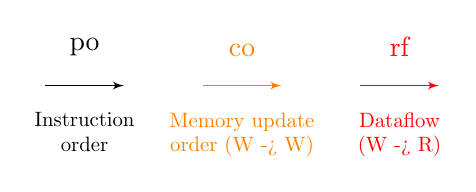
\begin{tikzpicture}[scale=1,every node/.style={transform shape},shift=({0, 1})]
        \tikzset{po_edge/.style = {->,> = latex',color=black}}
        \tikzset{hb_edge/.style = {->,> = latex',color=black,dashed}}
        \tikzset{ppo_edge/.style = {->,> = latex',color=gray}}
        \tikzset{rf_edge/.style = {->,> = latex',color=red}}
        \tikzset{fr_edge/.style = {->,> = latex',color=cyan}}
        \tikzset{co_edge/.style = {->,> = latex',color=orange}}
    
        \draw[po_edge,-] (0,0) edge [->] node[above=0.25cm]{po} node[below=0.25,scale=0.75,align=center]{Instruction\\order} (1,0); 
        \draw[co_edge,-] (2,0) edge [->] node[above=0.25cm]{co} node[below=0.25,scale=0.75,align=center]{Memory update\\order (W -> W)} (3,0); 
        \draw[rf_edge,-] (4,0) edge [->] node[above=0.25cm]{rf} node[below=0.25cm,scale=0.75,align=center]{Dataflow\\(W -> R)} (5,0); 
    \end{tikzpicture}    
    
    \textcolor{gray}{\smaller\\$\forall r^\x \exists w^\x: w^\x \mathcolor{red}{\xrightarrow{\mathit{rf}}} r^\x$\\$\forall w_1^\x, w_2^\x: w_1^\x \mathcolor{orange}{\xrightarrow{\mathit{co}}} w_2^\x \lor w_2^\x \mathcolor{orange}{\xrightarrow{\mathit{co}}} w_1^\x$\\$\dots$}
    
\end{subfigure}%
\hfill
\begin{subfigure}[c]{0.55\columnwidth}\centering
    \vspace{-0.5cm}
    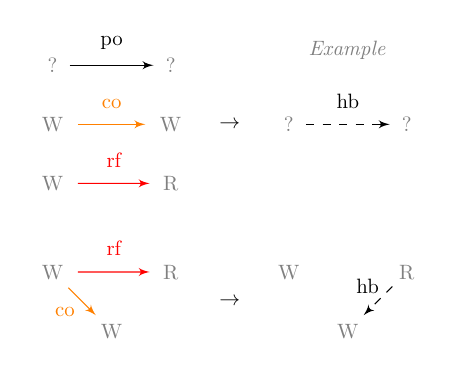
\begin{tikzpicture}[remember picture,scale=0.75,every node/.style={transform shape}]
        \tikzset{vertex/.style = {shape=ellipse,minimum size=1.5em,color=gray}}
        \tikzset{po_edge/.style = {->,> = latex',color=black}}
        \tikzset{hb_edge/.style = {->,> = latex',color=black,dashed}}
        \tikzset{ppo_edge/.style = {->,> = latex',color=gray}}
        \tikzset{rf_edge/.style = {->,> = latex',color=red}}
        \tikzset{fr_edge/.style = {->,> = latex',color=cyan}}
        \tikzset{co_edge/.style = {->,> = latex',color=orange}}

        \node[vertex] (ex) at (5, 0.25) {\emph{Example}};

        \node[vertex] (p0n0) at  (0,0) {?}; \node[vertex] (p0n1) at (2,0) {?}; \draw[po_edge] (p0n0) edge node[above=0.15cm]{po} (p0n1); 
        \node[vertex] (p1n0) at  (0,-1) {W}; \node[vertex] (p1n1) at (2,-1) {W}; \draw[co_edge] (p1n0) edge node[above=0.15cm]{co} (p1n1); 
        \node[vertex] (p2n0) at  (0,-2) {W}; \node[vertex] (p2n1) at (2,-2) {R}; \draw[rf_edge] (p2n0) edge node[above=0.15cm]{rf} (p2n1); 
        \node[] (label) at (3,-1) {$\rightarrow$};
        \node[vertex] (p0n2) at  (4,-1) {?}; \node[vertex] (p0n3) at (6,-1) {?}; \draw[hb_edge] (p0n2) edge node[above=0.15cm]{hb} (p0n3); 
        \node[vertex] (p3n0) at  (0,-3.5) {W}; \node[vertex] (p3n1) at (2,-3.5) {R}; \node[vertex] (p3n2) at (1,-4.5) {W}; \draw[rf_edge] (p3n0) edge node[above=0.15cm]{rf} (p3n1); \draw[co_edge] (p3n0) edge node[left,yshift=-5]{co} (p3n2); 
        \node[] (label) at (3,-4) {$\rightarrow$};
        \node[vertex] (p3n3) at  (4,-3.5) {W}; \node[vertex] (p3n4) at (6,-3.5) {R}; \node[vertex] (p3n5) at (5,-4.5) {W}; \draw[hb_edge] (p3n4) edge node[above,xshift=-5]{hb} (p3n5); 
    \end{tikzpicture}

    \begin{block}{}\smaller\centering
    Find \co{} and \rf{} for a given \po{} such that \hb{} is acyclic. 
    \end{block}

\end{subfigure}
\end{figure}
    \vspace{-3mm}
    \additionalSpace
}

\headerbox{example}{name=example,column=0,span=3}{
    \vspace{1.2mm}
    \begin{figure}[H]
\centering
\begin{subfigure}{0.5\columnwidth}
        \centering
            \begin{litmus}{2}{2w2r}{\x := 0, \y := 0}{\neg (i = 1 \land j = 0)}
                \x := 1 & i := \y\\
                \y := 1 & j := \x
            \end{litmus}
            \captionsetup{labelformat=empty}
            \caption{Program with property}
            \label{fig:example_program}
\end{subfigure}%
\begin{subfigure}{0.5\columnwidth}
            \centering
            \begin{execgraph}{1.25}
                \IW{\x}{0}
                \IW{\y}{0}
                
                \begin{thread}
                    \W{a1}{\x}{1}
                    \W{a2}{\y}{1}
                \end{thread}
                \begin{thread}
                    \R{b1}{\y}{i}
                    \R{b2}{\x}{j}
                \end{thread}
                
                \edge{po}{init}{a1}{}
                \edge{po}{init}{b1}{}
                \edge{po}{a1}{a2}{}
                \edge{po}{b1}{b2}{}
                \edgeL{rf}{init}{b2}{}{55}
                \edge{rf}{a2}{b1}{}
                
                \edgeR{co}{init}{a1}{}{20}
                \edgeR{co}{init}{a2}{}{55}

                \legend{po}
                \legend{rf}
                \legend{co}
                
            \end{execgraph}
            \captionsetup{labelformat=empty}
            \caption{CEx. candidate}
            \label{fig:example_candidate}

            
    \vspace{0.15cm}
            
\end{subfigure}
\captionsetup{labelformat=empty}
\caption{\textbf{Bold} variables are global, \emph{italicized} variables are local. The program is safe under SC and TSO but not PSO.}
\label{fig:example}
\end{figure}
    \vspace{-5mm}
    \additionalSpace
}

\headerbox{Tools for Weak Memory}{name=violation,column=0,span=4,below=overview}{
    \vspace{1.2mm}
    {
\vspace{1.4cm}
\centering
\smaller
\begin{columns}%
    \begin{column}{0.3\textwidth}%
        \centering
        
        \begin{block}{ \centering \bfseries
            Exhaustive Enumeration}

            Generate execution candidates, and check their consistency

        \end{block}

        \textbf{Herd7~\cite{herd}}\\{\smaller{(memory model simulator)}}
        
        Litmus tests
        CAT memory model         
        
    \end{column}%
    \hfill%
    \begin{column}{0.33\textwidth}%
        \centering

        \begin{block}{ \centering \bfseries
            Stateless Model Checking}
            
            Generate increasingly larger, always consistent executions (traces)

        \end{block}

        \textbf{GenMC~\cite{genmc}}, \textbf{Nidhugg~\cite{nidhugg}}, $\dots$\\{\smaller{}}

        
        (Subset of) C11
        
        Custom library

    \end{column}%
    \hfill%
    \begin{column}{0.3\textwidth}%
        \centering

        \begin{block}{ \centering \bfseries
            Bounded Model Checking}
            
            Encode constraints of the memory model in the SMT query
        
        \end{block}

        \textbf{Dartagnan~\cite{dartagnan}}

        (SV-COMP flavored) C
        
        Subset of CAT 
        

    \end{column}%
\end{columns}

\vspace{1.45cm}
}
    \vspace{-5mm}
    \additionalSpace
}

\headerbox{Violation Witness Example}{name=violationex,column=4,span=4,below=overview}{
    \vspace{1.2mm}
    \begin{table}[H]
\centering
\begin{tabular}{ccccc}
\textbf{Thread 0} & waypoint type & value & line & column \\\midrule
         & assume & $\backslash{}at(\x, 0) = 0$ & 0 & \emph{middle} \\
         & assume & $\backslash{}at(\y, 0) = 0$ & 0 & \emph{end} \\
         & thread\_start & 1, 2 & 1 & 0 \\
\textbf{Thread 1} & & &  &  \\\midrule
         & assume & $\backslash{}at(\x, 1) = 1$ & 1 & \emph{end} \\
         & assume & $\backslash{}at(\y, 1) = 1$ & 2 & \emph{end} \\
\textbf{Thread 2} & & &  &  \\\midrule
         & assume & $i = \backslash{}at(\x, 1)$ & 1 & \emph{end} \\
         & assume & $j = \backslash{}at(\y, 1)$ & 2 & \emph{end} \\
         & target & - & 2 & \emph{end} \\
\end{tabular}
\captionsetup{labelformat=empty}
\caption{A violation witness, encoding a violation under PSO}
\label{table:cex}
\end{table}
    \vspace{-5mm}
    \additionalSpace
}

\headerbox{Correctness Witness Example}{name=safetyex,column=0,span=4,below=violationex}{
    \vspace{1.2mm}
    \newcommand{\multiline}[1]{\begin{tabular}{c}#1\end{tabular}}

\begin{table}[H]
\centering
\begin{tabular}{ccccc}
invariant type & value & line & column \\\midrule
location & $\backslash{}at(\x, 0) = 0$ & 0 & \emph{middle} \\
location & $\backslash{}at(\y, 0) = 0$ & 0 & \emph{end} \\
         % & start & 1, 2 & 1 & 0 \\
% \textbf{Thread 1} & & &  &  \\\midrule
location & $\backslash{}at(\x, 1) = 1$ & 1 \emph{(left)} & \emph{end} \\
location & $\backslash{}at(\y, 1) = 1$ & 2 \emph{(left)} & \emph{end}\vspace{0.5em}\\
% \textbf{Thread 2} & & &  &  \\\midrule\vspace{0.5em}
location & \multiline{$\exists a : a \in \{0, 1\} $\\$i = \backslash{}at(\x, a)$}& 1 \emph{(right)} & \emph{end}\vspace{0.5em}\\
location & \multiline{$\exists a,b : a,b \in \{0, 1\} $\\$j = \backslash{}at(\y, a)$\\$i = \backslash{}at(\x, b)$\\$b = 1 \implies a = 1$} & 2 \emph{(right)} & \emph{end}\vspace{0.5em}\\
location & $\neg (i = 1 \land j = 0)$  & 2 \emph{(right)} & \emph{end} \\
\end{tabular}
\captionsetup{labelformat=empty}
\caption{A correctness witness, encoding a proof over SC}
\label{table:proof}
\end{table}
    \vspace{-5mm}
    \additionalSpace
}

\headerbox{Mapping Verdicts to Witnesses}{name=safety,column=4,span=4,below=violationex}{
    \vspace{1.2mm}
    $\backslash{}at(\mathbf{e}, \mathbf{id})$: Built-in ACSL construct \emph{(abused a bit)}
\begin{itemize}
    \item referring to the value of the expression \textbf{e} in the state at label \textbf{id}~\cite{ACSL}
    \item Our \emph{state labels} are integers, and denote ordering of memory events.
    \item Correctness: \emph{state labels} are \textbf{symbolic} integers, and denote ordering of memory events.
\end{itemize}

    \additionalSpace
}

\headerbox{Future Plans}{name=ourtools,column=4,span=4,below=safety}{
    \vspace{1.2mm}
    
\begin{itemize}
    \item Implement witness serialization (\textsc{Theta}, \textsc{CPAchecker})
    \item Implement violation witness checking (\textsc{Theta})
    \item Implement correctness witness checking (\textsc{Theta})
\end{itemize}

\begin{figure}[H]
\centering
\begin{subfigure}{0.5\columnwidth}
\centering

\end{subfigure}%
\begin{subfigure}{0.5\columnwidth}
            \centering
            

\includegraphics[width=0.75\textwidth]{logos/theta-logo.pdf}
            
\end{subfigure}
\end{figure}
    \additionalSpace
}

\headerbox{References}{name=references,column=0,span=7,below=safetyex}{
  \vspace*{-1.8mm}
  \begin{scriptsize}
  \begin{multicols}{2}
    \setlength{\bibsep}{0em}
    \renewcommand\refname{\vspace{-6.3mm}}
    \bibliographystyle{ftsrg-splncs04}
    \bibliography{poster}
  \end{multicols}
  \end{scriptsize}
}

\headerbox{Report}{name=qr,column=7,span=1,below=safetyex}{
  \centering
  
\includegraphics[width=\textwidth]{content/qr.pdf}
  \vspace*{-1cm}
}

\headerbox{}{name=ack,below=qr,boxheaderheight=0em,headerfont=\normalfont\bfseries\large,column=0,span=8,headerborder=none,textborder=none,headerColorOne=white,headerColorTwo=white,boxColorOne=white}{
\begin{spacing}{0.5}
{\smaller\smaller
This research was partially funded by the \'UNKP-24-3 New National Excellence Program of the Ministry of Innovation and Technology, from the National Research, Development and Innovation Fund of Hungary (grant no. \'UNKP-24-3-BME-213). 

The Doctoral Excellence Fellowship Programme (DCEP) is funded by the National Research Development and Innovation Fund of the Ministry of Culture and Innovation and the Budapest University of Technology and Economics, under a grant agreement with the National Research, Development and Innovation Office.

This project was funded in part by the Deutsche Forschungsgemeinschaft (DFG) --- \href{http://gepris.dfg.de/gepris/projekt/378803395}{378803395} (ConVeY)
}
\end{spacing}
}

\end{poster}

\end{document}